Une partie du concours sera réservée aux robots capables de suivre une ligne tracée au sol, indépendamment de tout contrôle humain. Si vous désirez y participer, vous trouverez ci-dessous les instructions pour la connexion du capteur et la programmation de l'Arduino. \\

Comme illustré à la Figure~\ref{fig:circuit}, la détection d'une ligne se fait à partir d'une LED et d'une photodiode. Le principe de base du fonctionnement est assez simple: la LED éclaire une surface et la photodiode mesure la partie de la lumière qui est réfléchie. En fonction de la couleur de la surface, plus ou moins de lumière sera réfléchie, ce qui permet donc de déterminer si on est au-dessus d'une ligne noire ou au-dessus d'une surface blache à partir de la mesure de la photodiode.\\

La façon dont le circuit de lecture de la photodiode fonctionne est un peu plus subtile. Les plus attentifs auront peut-être remarqué que la diode semble être branchée à l'envers, dans le sens non-passant avec la cathode du côté positif et l'anode du côté négatif. Du coup, comment fait-on pour effectuer une mesure si aucun courant ne passe? En réalité, quand une diode est branchée dans le sens non-passant, un courant très faible passe néanmoins. Dans une photodiode, ce courant va dépendre de la quantité de lumière reçue dans un certain intervalle de longueurs d'ondes (dans notre cas pour des lumières infrarouges). Ce courant qui varie, de l'ordre de quelques nA dans le noir à plusieurs $\mu$A à la lumière, passe à travers une résistance, ce qui crée donc une variation de la différence de potentiel. En lisant la tension grâce à l'ADC de l'Arduino sur la broche A0, on peut donc détecter un changement de lumière.\\

\begin{figure}[!t]
\centering
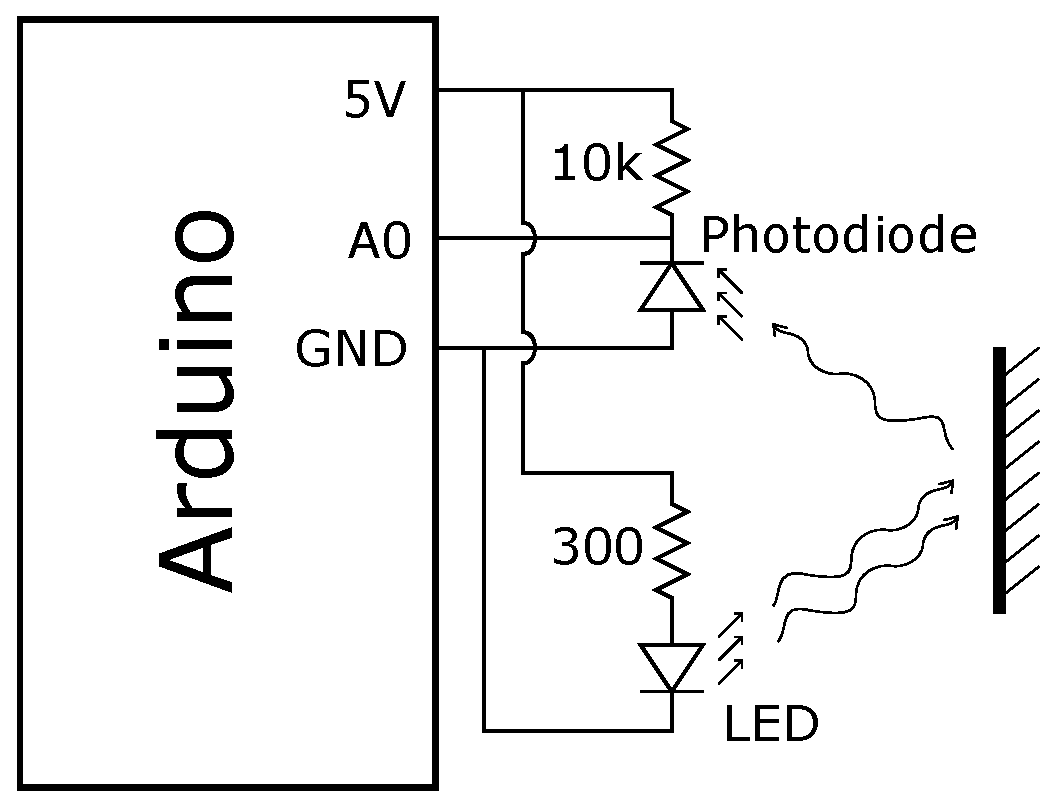
\includegraphics[width=0.4\textwidth]{imgs/circuit.eps}
\caption{Circuit et principe de fonctionnement pour la détection de ligne.}
\label{fig:circuit}
\end{figure}

Dans le code, la lecture de la tension se fait grâce à la fonction \textit{analogRead(pin)}. Vous pouvez faire l'essai avec le morceau de code ci-dessous. Observez le changement de ce qui s'affiche dans le terminal en fonction de la surface qui fait face au capteur. 

\lstset{language=C}
\begin{lstlisting}[frame=single,numbers=left,numberstyle=\small,label={code1},caption={Lecture de la photodiode.}]
const int PHOTO_PIN = 14;

int val = 0; 

void setup() {
  Serial.begin(9600); 
}

void loop() {
  val = analogRead(analogPin);  
  Serial.println(val);      
  delay(300);
}

\end{lstlisting}

A partir de cette valeur, vous pouvez maintenant essayer de programmer le contrôle du mouvement de votre robot. Il existe énormément de stratégies possibles, des très simples aux plus compliquées, avec un ou plusieurs capteurs. A vous de réfléchir à ce que votre robot doit viser comme valeur sur les capteurs, quand et comment tourner pour rester le plus proche possible de la ligne... Pour vous aider, n'hésitez pas à aller faire un tour sur Internet, certains projets en ligne pourront probablement vous aider!